\pdfoutput=1

\documentclass[12pt, a4paper]{article}
\usepackage[utf8]{inputenc}

\usepackage[style= bwl-FU, backend = biber, maxbibnames=99, maxcitenames=2,uniquelist=minyear, firstinits=true]{biblatex}

% \AtEveryBibitem{\clearfield{number}}
% \AtEveryBibitem{\clearfield{doi}}
\AtEveryBibitem{\clearfield{note}}
\AtEveryBibitem{\clearfield{urldate}}
\AtEveryBibitem{\clearfield{issn}}
\AtEveryBibitem{\clearfield{isbn}}
%
\addbibresource{Library.bib}

\usepackage{authblk}
\usepackage{color,graphicx,tikz}
\usetikzlibrary{positioning,arrows}
% The amssymb package provides various useful mathematical symbols
\usepackage{mathtools,amssymb,amsmath,mathdots,amsfonts}
\usepackage[mathscr]{eucal} %just for the font \mathscr
\usepackage{enumerate}
%\usepackage{amsthm}
%\usepackage{mathaccents}
\usepackage{setspace}
\newtheorem{remark}{Remark} [section]
\usepackage{hyperref}

% macros used across many documents for multiple scattering notation
%% Packages for commenting and striking through text %%%%
\usepackage[colorinlistoftodos,bordercolor=orange,backgroundcolor=orange!20,linecolor=orange,textsize=scriptsize]{todonotes}
\usepackage{soul}
\newcommand{\will}[1]{\todo[inline]{\textbf{Will: }#1}}
\newcommand{\art}[1]{\todo[inline]{\textbf{Artur: }#1}}
\newcommand{\david}[1]{\todo[inline]{\textbf{David: }#1}}
\newcommand{\mike}[1]{\todo[inline]{\textbf{Mike: }#1}}
\newcommand{\wrong}[1]{\textcolor{red}{\st{#1}}}
%%%--------------------------------------------------%%%

\newcommand \eff {*}
\newcommand \scatZ {Z}
\newcommand \scatZs {\zeta}
\newcommand \Q {\vec Q}
\newcommand \T {\vec T}
\newcommand \B {\mathcal B}
\newcommand \regS {\mathcal S}
\newcommand \M {\vec {\mathcal M}}
\newcommand \s {\mathbf s}
\newcommand \Ab {\mathcal A}
\newcommand \A [1] {\Ab_#1}
\newcommand \p {p}
\newcommand \prob {P}
\newcommand {\type} [1]{{\{#1\}}}
\newcommand \reg {\mathcal R_N}
\newcommand \reginf {\mathcal R_\infty}
\newcommand {\nfrac}[1] {\mathfrak n_{#1}}
\newcommand {\Lamo}{\vec \Lambda}
\newcommand {\Lam}[1]{\Lamo_{#1}}
\newcommand \ef{\mathrm{E}}
\newcommand \reflect{\mathrm{ref}}
\newcommand \inc{\mathrm{in}}
\newcommand \In{\mathrm{I}}
\newcommand \cs { S}
\newcommand \cl { L}
\newcommand \Out{\mathrm{o}}

% \newcommand \nfrac {\mathfrak n_0}
\newcommand{\ensem}[1]{\langle #1 \rangle}

\def\bga#1\ega{\begin{gather}#1\end{gather}} % suggested in technote.tex
\def\bgas#1\egas{\begin{gather*}#1\end{gather*}}

\def\bal#1\eal{\begin{align}#1\end{align}} % suggested in technote.tex
\def\bals#1\eals{\begin{align*}#1\end{align*}}

\renewcommand{\vec}[1]{\boldsymbol{#1}}
\renewcommand{\thefootnote}{\fnsymbol{footnote}}

\newcommand{\initial}[1]{{#1}_\circ}
\newcommand{\ii}{\textrm{i}}
\newcommand{\ee}{\textrm{e}}
\newcommand{\deriv}[2]{\frac{\partial{#1}}{\partial{#2}}}
\newcommand{\derivtwo}[2]{\frac{\partial^{2}{#1}}{\partial{#2}^2}}
\newcommand{\derivtwomix}[3]{\frac{\partial^{2}{#1}}{\partial{#2}\partial{#3}}}

\newcommand{\bb}{\mathcal B}
\newcommand{\R}{\mathbb{R}}
\newcommand{\filler}{\hspace*{\fill}}

\newcommand{\lit}{\hspace{0.2cm}}

\newtheorem{theorem}{Theorem}
\def \proof{\noindent {\bf \emph{Proof:}} }


% \DeclareMathOperator{\sign}{sgn}
% \DeclareMathOperator{\divergence}{div}
% \DeclareMathOperator{\tr}{tr}
% \DeclareMathOperator{\Ord}{\mathcal{O}}
% \DeclareMathOperator{\GRAD}{grad}
% \DeclareMathOperator{\DIV}{DIV}
% \DeclarePairedDelimiter{\ceil}{\lceil}{\rceil}


%%% Local Variables:
%%% mode: latex
%%% TeX-master: t
%%% End:


% \graphicspath{{../images/}}
%\graphicspath{{Media/}}

\doublespacing
% \setlength{\topmargin}{0cm} \addtolength{\textheight}{2cm}
\evensidemargin=0cm \oddsidemargin=0cm \setlength{\textwidth}{16cm}

\begin{document}

\title{Numerically solving integral equations of wave ensembles}

% \author{
% Artur L. Gower$^{a}$, Michael J. A. Smith$^{a}$, \\ William Parnell$^{a}$ and David Abrahams$^{a,b}$ \\[12pt]
% \footnotesize{$^{a}$ School of Mathematics, University of Manchester, Oxford Road, Manchester, M13 9PL, UK}\\
% \footnotesize{$^{b}$ Isaac Newton Institute for Mathematical Sciences, 20 Clarkson Rd, Cambridge CB3 0EH, UK}
% }

\author[$\dagger$]{Artur L.\ Gower}

\affil[$\dagger$]{School of Mathematics, University of Manchester, Oxford Road, Manchester M13 9PL, UK}

\date{\today}
\maketitle

\begin{abstract}
Allows for a broad frequency range, and to easily test different statistical assumptions. Assumptions such as the pair-correlation and QCA.
\end{abstract}

\noindent
{\textit{Keywords:} polydisperse, multiple scattering, Fredholm Integral equations, multi-species, effective waves, quasicrystalline approximation, statistical methods}


\section{Effective waves for uniformly distributed species}
\label{sec:results}

We consider a halfspace $x>0$ filled with $S$ types of inclusions (species) that are uniformly distributed. The fields are governed by the scalar wave equation:
\begin{align}
  &\nabla^2 u + k^2 u = 0, \quad \text{(in the background material)} \\
  &\nabla^2 u + k^2_j u = 0, \quad \text{(inside the $j$-th scatterer)},
\end{align}
 The background and species material properties are summarised in Table~\ref{tab:properties}.
The goal is to calculate how a medium with these scatterers, randomly uniformly distributed, reflects and transmits waves in an
\href{https://en.wikipedia.org/wiki/Ensemble_average_(statistical_mechanics)}{ensemble average sense}.

For simplicity we will consider that all particles are cylindrical, though it is easy to extend the results to any smooth particle by using Waterman's T-matrix\cite{waterman_symmetry_1971,varadan_multiple_1978,mishchenko_t-matrix_1996}.

\begin{table}[h]
\centering
\begin{tabular}{|l| l|}
  \hline
Background properties: &  wavenumber $k$ \hspace{0.8cm} density $\rho$  \hspace{0.25cm} sound speed $c$
\\ \hline
Specie properties: & number density $\nfrac j$ \hspace{0.1cm} density $\rho_j $
\hspace{0.1cm} sound speed $c_j$  \hspace{0.1cm} radius $a_j$
\\\hline
\multicolumn{2}{|l|}{
  total number density $\nfrac {}$   \hspace{0.2cm}  effective wavenumber $k_\eff$ \hspace{0.2cm} species min. distance $a_{j\ell} > a_j + a_\ell$
}
\\\hline
% 2D Incident wave & $u_\inc(x,y) = \ee^{\ii \mathbf k \cdot \mathbf x} \quad \text{with} \quad \mathbf k \cdot \mathbf x = k x \cos \theta_\inc  + k y \sin \theta_\inc $
\end{tabular}
\label{tab:properties}
\caption{Summary of material properties and notation. The index $j$ refers to properties of the $j$-th species. Note a typical choice for $a_{j\ell}$ is $a_{j\ell} = c (a_j + a_\ell)$, where $c=1.01$.}
\end{table}


\section{Cylindrical species}

We consider an incident wave
\begin{gather}
  u_\inc =  \ee^{\ii \mathbf k \cdot \mathbf x} \quad \text{with} \quad \mathbf k \cdot \mathbf x = k x \cos \theta_\inc  + k y \sin \theta_\inc,
%   u_\inc(x,y) = \ee^{\ii \mathbf k \cdot \mathbf x}, \quad \text{with} \quad \mathbf k \cdot \mathbf x = \alpha  x  + \beta y,
% \notag \\
%   \text{where} \qquad  \alpha = k \cos \theta_\inc, \quad \beta = k \sin \theta_\inc,
  \label{eqns:incident}
\end{gather}
and angle of incidence $\theta_\inc$ from the $x$-axis, exciting a material occupying the halfspace $x>0$.

Combining equations (3.6) and the quasicrystalline approximation (3.10) from \parencite{gower_reflection_2018}, we arrive at
\begin{multline}
 \sum_{n=-\infty}^\infty \int_\regS \int_{\stackrel{x_2 > 0 }{\|\mathbf x_1 - \mathbf x_2 \| > a_{12}}}  \A n (k \mathbf x_2, \s_2) F_{n-m}(k\mathbf x_2 - k \mathbf x_1,k)  d \mathbf x_2 d\s_2^n
\\
+  \A m (k\mathbf x_1, \s_1) + \ee^{\ii \mathbf x_1 \cdot \mathbf k } \ee^{\ii m ( \pi/2 - \theta_\inc )}
   = 0, \quad \text{for} \quad x_1 >0,
  \label{eqn:ensemAsystem}
\end{multline}
where
\begin{align}
  & d\s_2^n = \nfrac {} \scatZ_n (\s_2) p(\s_2) d\s_2,
  \\
  & F_{n}(\mathbf X,k) = (-1)^{n}\ee^{\ii n \Theta} H_{n}(R)( 1 + g(R/k;  \s_1,\s_2)),
  \label{eqn:integral_kernel}
\end{align}
with $(R,\Theta)$ being the polar coordinates of $\mathbf X = (X,Y)$,
$p(\s_1)$ is the probability density function of picking a species in $\regS$ and we assumed statistical independence $p(\s_1, \s_2) = p(\s_1)p(\s_2)$. Note we included $k$ in the argument of $\A m$ for convenience, as later we will non-dimensionalise. The function $g(R; \s_1,\s_2)$ is the pair-correlation, assuming $R$ is the distance between two particles, one centred of type $\s_1$ and another of type $\s_2$. If we were to use whole correction, then $g(R; \s_1,\s_2) = 0$.
For most random systems we expect that rapidly $g(R; \s_1,\s_2) \to 0$ as $R \to \infty$, so we will assume
\begin{equation}
  g(R; \s_1,\s_2) = 0, \quad \text{ for } \; R > \bar a_{12}.
  \label{eqn:pair_correlation}
\end{equation}
In terms of the notation from \parencite{gower_reflection_2018}:
\begin{multline}
  |\reg| p(\Lam 2 | \Lam 1) = |\reg|^2 \frac{p(\Lam 1, \Lam 2)}{p(\s_1)} = |\reg|^2 p(\s_2) p(\mathbf x_1, \mathbf x_2 | \s_1,\s_2)
  \\ = p(\s_2)(1 + g(\|\mathbf x_1 - \mathbf x_2\|;  \s_1,\s_2)).
\end{multline}

For computational efficiency, we will change variables to
\begin{align}
& X = k\mathbf x_2 - k\mathbf x_1, \quad (x,y) = (kx_1,ky_1),
% \\
% & b = a_{12}}, \quad  \bar b = \bar a_{12}}, \quad  \s_2 = \s_2, \quad  \s_1 = \s_{},
\end{align}
% where the last line is just to have a consistent notation.
We also borrow equation (4.1) from \parencite{gower_reflection_2018} to substitute
\begin{equation}
  \A m (k x_1, k y_1, \s) = \A m (k x_1, \s) \ee^{\ii k y_1 \sin\theta_\inc},
  \label{eqn:A_symmetry}
\end{equation}
which is due to the symmetry of~\eqref{eqn:ensemAsystem}. Substituting the above into~\eqref{eqn:ensemAsystem}, we can rewrite the integrated term:
\begin{multline*}
     \int_{\stackrel{x_2 > 0 }{\|\mathbf x_2-\mathbf x_1 \| > a_{12}}} \A n (k x_2, \s_2) \ee^{\ii y_2 k \sin\theta_\inc} F_{n-m}(k\mathbf x_2 - k \mathbf x_1,k) d \mathbf x_2 =
  \\
   \frac{\ee^{\ii y \sin\theta_\inc}}{k^2} \int_{X> -x} \A n (X + x, \s_2) \int_{Y^2 > k^2 a_{12}^2 - X^2}
   \ee^{\ii Y \sin\theta_\inc} F_{n-m}(\mathbf X,k) d Y d X,
\end{multline*}
then we split the integral on the right in the form
\begin{align*}
  &\int_{Y^2 > k^2 a_{12}^2 - X^2} \ee^{\ii Y \sin\theta_\inc} F_{n-m}(\mathbf X,k) d Y
 = \chi_{\{ |X|< k a_{12}\}} B_{n-m}(X,k)
   +  \chi_{\{ |X|> k a_{12}\}}S_{n-m}(X,k),
\end{align*}
where by using~\eqref{eqn:pair_correlation}, equation (B.3) from \cite{gower_reflection_2018},
\begin{equation}
  S_n(X,k) =  \int_{-\infty}^\infty \ee^{\ii Y \sin\theta_\inc}
  F_{n}(\mathbf X,k) d Y =
G_{n}(X, k) +
\frac{2}{\cos \theta_\inc}
\begin{cases}
  \ii^{n} \ee^{-\ii n \theta_\inc} \ee^{\ii X \cos \theta_\inc } & X \geq 0,\\
  (-\ii)^{n} \ee^{\ii n \theta_\inc} \ee^{-\ii X \cos \theta_\inc } & X < 0,
\end{cases}
  % \int_{-\infty}^\infty \ee^{\ii y_2 k \sin\theta_\inc} \ee^{\ii (n-m) \Theta_{12}} H_{n-m}(k R_{12})d y_2
  % \\
  % + (-1)^{n-m} \int_{y_2 \in B(\bar a_{12}})} \ee^{\ii y_2 k \sin\theta_\inc} \ee^{\ii (n-m) \Theta_{12}} H_{n-m}(k R_{12})g(\|\mathbf x_1 - \mathbf x_2\|;  \s_1,\s_2) d y_2
  \label{eqn:Sn}
\end{equation}
 with
\begin{multline}
G_n(X, k) = (-1)^{n} \int_{-\sqrt{k^2 \bar a_{12}^2 - X^2}}^{\sqrt{k^2\bar a_{12}^2 - X^2}} \ee^{\ii Y \sin\theta_\inc}
  \ee^{\ii n \Theta} H_{n}(R)g(R/k;  \s_1,\s_2) d Y
  \\ = 2 (-1)^{n} \int_{0}^{\sqrt{k^2\bar a_{12}^2 - X^2}} \cos\left(Y \sin\theta_\inc + n \Theta\right) H_{n}(R)g(R/k;  \s_1,\s_2) d Y
\end{multline}
The term
\begin{multline}
  B_n(X,k) = \int_{-\infty}^{\infty} \chi_{\{ Y^2> k^2 a_{12}^2 - X^2\}} \ee^{\ii Y \sin\theta_\inc}
   F_{n}(\mathbf X,k) d Y
  \\
  = 2(-1)^{n} \int_{\sqrt{k^2 a_{12}^2 - X^2}}^\infty \cos \left( Y \sin\theta_\inc +  n \Theta\right) H_{n}(R)( 1 + g(R/k;  \s_1,\s_2)) d Y.
\end{multline}
It is difficult to numerically integrate the above because the integrand tends to zero very slowly as $Y$ increases. To numerically integrate the above we use
\begin{align}
  & \cos \left( Y \sin\theta_\inc +  n \Theta\right) = \cos((n \pi)/2 + Y \sin(\theta_\inc)) + \mathcal O(X/Y),
  \\
  & H_{n}(R) =  -(-1)^{3/4} \ee^{-\ii n \pi /2} \sqrt{\frac{2}{\pi Y}} + \mathcal O(X^{3/2}/Y^{3/2}),
\end{align}
which we use to rewrite
\begin{multline}
  B_n(X,k) = 2(-1)^{n} \int_{\sqrt{k^2 a_{12}^2 - X^2}}^{Y_1} \cos \left( Y \sin\theta_\inc +  n \Theta\right) H_{n}(R)( 1 + g(R/k;  \s_1,\s_2)) d Y
  \\ + \frac{1 + \ii}{\sqrt{\pi Y_1} \cos(\theta_\inc)^2} \ee^{\ii  Y_1 (1 - \sin(\theta_\inc))}
  \left[ 1 + (-1)^n \ee^{2 \ii Y_1 \sin(\theta_\inc)} (1 - \sin(\theta_\inc)) + \sin(\theta_\inc) \right] + \mathcal O(X/Y),
\end{multline}
where we assumed that $g(R/k;  \s_1,\s_2) =0$ for $Y>Y_1$.

Written in full the governing equation~\eqref{eqn:ensemAsystem} now becomes
\begin{multline}
 \sum_{n=-\infty}^\infty \int_\regS
  \int_{X> 0} \A n (X, \s_2) K(X - x,k) dX
  d\s_2^n
\\
+  k^2 \A m (x, \s_1)   + k^2  \ee^{\ii x \cos \theta_\inc} \ee^{\ii m ( \pi/2 - \theta_\inc )}
   = 0, \quad \text{for} \quad x_1 >0,
  \label{eqn:ensemAsystem2}
\end{multline}
where I swapped the integration variable $X \to X - x$.
% Uncomment to see in full
% \begin{align*}
%    \frac{k^2}{\ee^{\ii y \sin\theta_\inc}} & \int_{\stackrel{x_2 > 0 }{\|\mathbf x_2-\mathbf x_1 \| > a_{12}}} \A n (x_2, \s_2) \ee^{\ii y_2 k \sin\theta_\inc} F_{n-m}(k\mathbf x_2 - k \mathbf x_1,k) d \mathbf x_2
%   \\
%   &=\int_{X> -x} \A n (X/k + x/k, \s_2)
%   \chi_{\{ |X|< k a_{12}\}}   B_{n-m}(X,k)
%    d X,
%   \\
%   & +\int_{X> -x} \A n (X/k + x/k, \s_2)
%   \chi_{\{ |X|> k a_{12}\}} \left [G_{n-m}(X, k) + \frac{2 \ii^{n-m} \ee^{-\ii(n-m) \theta_\inc}}{\cos \theta_\inc} \ee^{\ii X \cos \theta_\inc } \right ]
%    d X,
% \end{align*}
where
\begin{equation}
K(X-x,k) =   \chi_{\{ |X-x|> k a_{12}\}}  S_{n-m}(X-x,k)
% \left [G_{n-m}(X-x, k) + \frac{2 \ii^{n-m} \ee^{-\ii(n-m) \theta_\inc}}{\cos \theta_\inc} \ee^{\ii (X - x) \cos \theta_\inc } \right ]
% \\
 + \chi_{\{ |X - x|< k a_{12}\}}   B_{n-m}(X- x,k).
\label{eqn:kernel}
\end{equation}
% Numerically it is better to substitute in the above to reach
% \begin{multline}
%   \sum_{n=-\infty}^\infty \int_\regS
%   \int_{\stackrel{|X-x|> k a_{12}}{X>0}} \A n (X/k, \s_2) S_{n-m}(X-x, k) dX
%   d\s_2^n
%   \\
%   +  \sum_{n=-\infty}^\infty \int_\regS
%     \int_{\stackrel{|X-x| < k a_{12}}{X>0}} \A n (X/k, \s_2) B_{n-m}(X- x,k) dX
%     d\s_2^n
% \\
% +  k^2 \A m (x/k, \s_1)   + k^2  \ee^{\ii x \cos \theta_\inc} \ee^{\ii m ( \pi/2 - \theta_\inc )}
%    = 0, \quad \text{for} \quad x_1 >0,
%   \label{eqn:ensemAsystem3}
% \end{multline}
\subsection{Numerical solution}
\label{sec:numerical}

To start we consider only one single species and consider only whole correction pair-correlation. After trying methods based on Chebyshev and function approximation, I've decided they are too computationally intense. For this reason I'm going with the simple discretisation: $\A n^j = \A n (x^j)$ for $x^j = j h$ and $j=0,\ldots,J$. A regular spaced mesh is best for convolutions. With analogous notation for the other fields, let the vectors:
\begin{equation}
  \vec \Ab_n = (\Ab_n^j)_j, \quad \vec S_n = (S_n^j)_j, \quad \vec B_n = (B_n^j)_j, \quad \vec b_n = - k^2(\ee^{ \ii x^j \cos \theta_\inc} \ee^{\ii n ( \pi/2 - \theta_\inc )})_j.
  \label{eqns:discretisation}
\end{equation}


\begin{multline}
  \sum_{n=-\infty}^\infty
  \int_\regS \int_{X>0} \A n (X) S_{n-m}(X-x) dX
  d\s_2^n
  \\
  +  \sum_{n=-\infty}^\infty
    \int_\regS \int_{\stackrel{|X-x| < k a_{12}}{X>0}} \A n (X) (B_{n-m}(X- x,k) - S_{n-m}(X-x) )dX
    d\s_2^n
\\
+  k^2 \A m (x)   + k^2  \ee^{\ii x \cos \theta_\inc} \ee^{\ii m ( \pi/2 - \theta_\inc )}
   = 0, \quad \text{for} \quad x_1 >0
  \label{eqn:ensemAsystem4}
\end{multline}

\art{as the integrals are convolutions, it may be possible to use a Fourier of Laplace transform to solve this.}
Now considering only one species (to reduce the number of sums)
\begin{equation}
  \nfrac {} \sum_{n,j \geq 0}  \scatZ_n  \sigma_j  \left ( S_{n-m}^{j-\ell}
  +  (B_{n-m}^{j-\ell} - S_{n-m}^{j -\ell} ) \chi_{\{|j-\ell|\leq p\}} \right) \Ab_n^j+  k^2  \Ab_m^\ell  =  b_m^\ell,
  \label{eqn:ensemAsystemN}
\end{equation}

\art{the above discrete integrals have been checked against Mathematica brute force numerical evaluation.}
for $\ell >0$, where $p = \lfloor k a_{12}/h \rfloor$, and $\sigma_j$ represents the discrete integral. In matrix form,
\begin{equation}
  % \nfrac {} \sum_{n}  \scatZ_n  \overset{\infty}{\vec P}_{n-m} \overset{\infty}{\vec \Ab}_n
  \sum_{n} \vec {\mathcal E}_{nm}
+ \nfrac {} \sum_{n}  \scatZ_n ( \vec P_{n-m} + \vec Q_{n-m}) \vec \Ab_n
+  k^2 \vec I \vec \Ab_m  =  \vec b_m,
  \label{eqn:ensemAsystemN2}
\end{equation}
where the components of matrices are
\begin{equation}
  P_{n}^{\ell j} =  \sigma_j S_{n}^{j-\ell}, \quad Q_{n}^{\ell j} = \sigma_j (B_{n}^{j-\ell} - S_{n}^{j -\ell} ) \chi_{\{|j-\ell| \leq p\}},
\end{equation}
with $j,\ell = 0,1, \ldots, J$
% The $\infty$ over a symbol, such $(\overset{\infty}{\vec P}_{n})^{\ell j} = P_{n}^{\ell j}$ and $(\overset{\infty}{\vec \Ab}_{n})^{\ell j} = \Ab_{n}^{\ell j}$, indicate that $j,\ell = J+1,J+2, \ldots, \infty$
, and
\begin{equation}
  \mathcal E_{nm}^\ell  = \nfrac {} Z_n \int_{X> x^J} \A n (X) S_{n-m}(X-x^\ell) dX. %\quad \text{with} \;\; \bar x = Jh.
  \label{eqn:E}
\end{equation}
If we do not include $\mathcal E_{nm}^\ell$, then the solution of \eqref{eqn:ensemAsystemN2} would be valid for a plate occupying the region $0 \leq x \leq x^J$. If we wish to calculate the backscattering from the whole halfspace, then we can calculate $\mathcal E_{nm}^\ell$ by approximating $\Ab_n(x)$ as a sum of plane waves, shown below.

\subsection{Effective waves}
The average scattering coefficients can be approximated by a sum of plane waves:
\begin{equation}
  \Ab_n(X) = \ii^n \sum_p \ee^{-\ii n \theta_p} A_{n}^p \ee^{\ii (X -\bar x) \frac{k_p}{k} \cos \theta_p } \quad \text{for} \;\; X > \bar x ,
\label{eqn:effective_waves}
\end{equation}
where $\bar x$ is for now undetermined, except $\bar x < x^J$, so that the above has a region of overlap with the discrete form~\eqref{eqns:discretisation}. For each $p$ the terms $A^p_n$ and $k_p$ satisfy the dispersion equation
\begin{equation}
  \sum_n D_{nm}(k_p) A^p_n =0,
  \label{eqn:dispersion}
\end{equation}
for all $m$. We can then determine $k_p$ by solving $\det (D_{nm}(k_p)) =0$, where we require
$\text{Im} \;  k_p > 0$ to guarantee that the integral~\eqref{eqn:E} converges, and to lead to a physically reasonable solution. The components $D_{nm}$ are given by... Once $k_p$ is determined,then~\eqref{eqn:dispersion} can be used to write the vector $ \mathbf A^p = [\ldots, A^p_{-n}, A^p_{1-n}, \ldots, A^p_{n-1}, A^p_{n}, \ldots]$ in the form
\begin{equation}
  \mathbf A^p = \alpha^p \mathbf a^p,
  \label{eqn:A_eigenvector}
\end{equation}
 where $\mathbf a^p$ is determined from~\eqref{eqn:dispersion} and $\alpha^p$ is unknown. With $k_p$, we can also determine the angle $\theta_p$ by using Snell's law: $k_p \sin \theta_p = k \sin \theta_\inc$. From here onwards, we assume that $k_p$, $\theta_p$ and the $\mathbf a^p$ have been determined.

 The average wave~\eqref{eqn:effective_waves} also needs to satisfy (extinction of the incident wave)
 \begin{multline}
 \sum_{n=-\infty}^\infty \frac{2 k \nfrac {} Z_n}{\cos \theta}  \sum_{p}
  A_n^p  \frac{\ee^{\ii n (\theta_\inc - \theta_p)} \ee^{ - \ii \bar x  \cos \theta}}{k_p \cos \theta_p - k \cos \theta}
   = \\
 \ii k^2 +  \frac{2\ii \nfrac {}}{\cos \theta} \sum_{n=-\infty}^\infty \int_{0}^{{\bar x}}
     \A n(X) Z_n (-\ii)^{n} \ee^{\ii n \theta_\inc} \ee^{-\ii X \cos \theta_\inc}  d X
     \\
   = \ii k^2 +
   \ii \nfrac {} \sum_{n=-\infty}^\infty Z_n \int_{0}^{{\bar x}}
     \A n(X) S_n(-X) d X.
     \label{eqn:extinction}
 \end{multline}
 For direct backscattering, $\theta_\inc = \theta_p =0$, we reach a simpler form:
 \begin{equation}
 \sum_{n=-\infty}^\infty 2 k \nfrac {} Z_n  \sum_{p}
  A_n^p  \frac{\ee^{- \ii \bar x}}{k_p  - k }
   = \ii k^2 +
   \ii \nfrac {} \sum_{n=-\infty}^\infty Z_n \int_{0}^{{\bar x}}
     \A n(X) S_n(-X) d X.
 \end{equation}
 Using~\eqref{eqn:A_eigenvector}, the discrete version of~\eqref{eqn:extinction} becomes
 \begin{align}
   &   \sum_p   W^p  \alpha^p - \ii \nfrac {} \sum_n Z_n \sum_{j=0}^L \sigma_j S^{-j}_n \Ab_n^j  =
   \ii k^2 \implies   \\ &
    \mathbf W \cdot \vec \alpha - \sum_n \vec{V}_n \cdot \vec \Ab_n =
    \ii k^2,
    \label{eqn:extinction_vector}
 \end{align}
 where $x^L = h L = \bar x \leq x^J$ and
 \begin{equation}
   W^p  = \sum_{n=-\infty}^\infty \frac{2 k \nfrac {} Z_n}{\cos \theta}
     \frac{\ee^{\ii n (\theta_\inc - \theta_p)} \ee^{- \ii \bar x  \cos \theta}}{k_p \cos \theta_p - k \cos \theta} a_n^p,  \quad
    V_n^j =  \ii \nfrac {} Z_n \sum_{j=0}^L \sigma_j S^{-j}_n.
    \label{eqn:extinction_matrix}
 \end{equation}
To determine the $\alpha^p$ we have so far only the scalar equation~\eqref{eqn:extinction_vector}. To completely determine the $\alpha^p$ (assuming there is more than one), we need to match the ansatz~\eqref{eqn:effective_waves} with the numerical solution introduced in Section~\ref{sec:numerical}.


\subsection{Connecting the integral and ansatz approach}

\begin{figure}
  \centering
  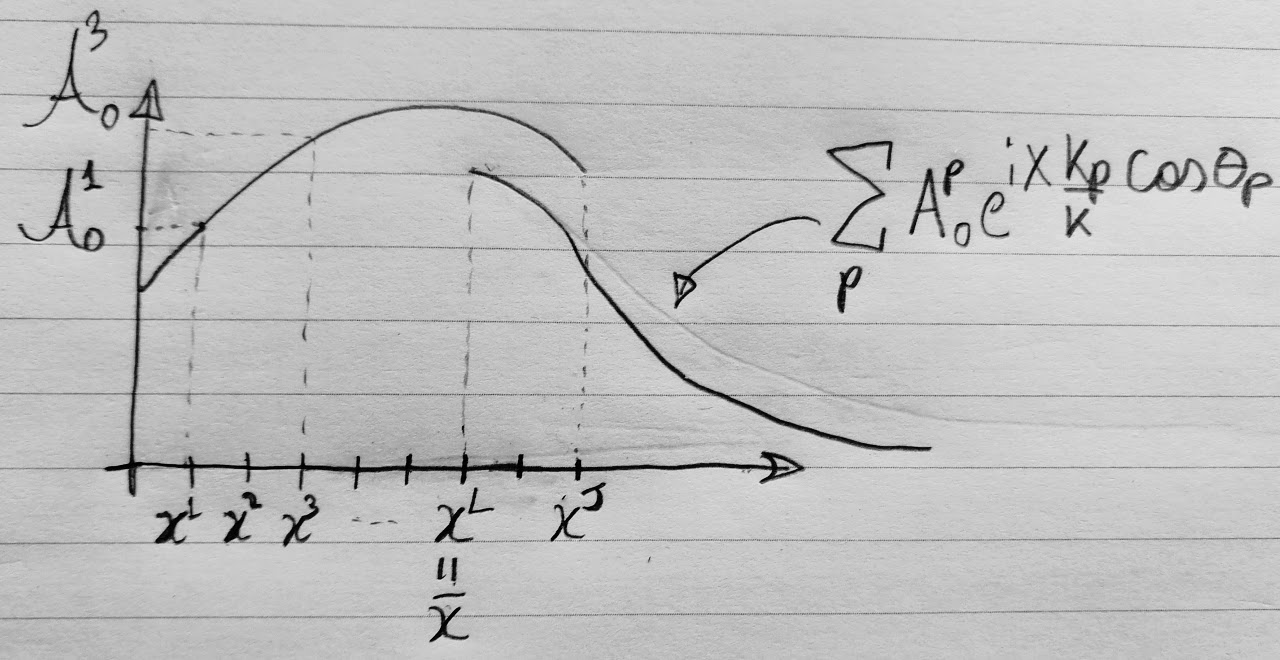
\includegraphics[width=0.8\linewidth]{connect_effective.jpg}
  \caption{Shows the overlap region of the numerical solution and the ansatz approach.}
  \label{fig:connect_effective}
\end{figure}

 Substituting~\eqref{eqn:effective_waves} into~\eqref{eqn:E} and using~\eqref{eqn:Sn} we arrive at
\begin{multline}
  % E_{n,m}^\ell  = \int_{X>x^J} \A n (X) S_{n-m}(X-x^\ell) dX  d\s_2^n.
  \mathcal E_{nm}^\ell  = \frac{2 \nfrac {} Z_n}{\cos \theta_\inc} (-1)^n \ii^{-m} \ee^{\ii (m-n) \theta_\inc}
   \sum_p \ee^{-\ii n \theta_p} A_{n}^p \int_{X> x^J} \ee^{\ii (X - \bar x)\frac{k_p}{k} \cos \theta_p +  \ii X\cos \theta_\inc}
  \ee^{- \ii x^\ell\cos \theta_\inc}
   dX
   \\
   = \frac{2 k \nfrac {} Z_n }{\cos \theta_\inc} (-1)^n \ii^{-m}
    \sum_p A_{n}^p \ee^{\ii (m-n) \theta_\inc - \ii n \theta_p}
    \frac{\ii \ee^{  \ii (x^J - \bar x)\frac{k_p}{k}  \cos \theta_p  + \ii  (x^J - x^\ell) \cos \theta_\inc }}
    {k_p \cos \theta_p + k\cos \theta_\inc},
    \label{eqn:E_eff}
\end{multline}
where we used $ X -x^\ell > x^J - x^\ell \geq 0$, for $\ell < J$, when substituting $S_{n-m}(X-x^\ell)$ with~\eqref{eqn:Sn}. Above we can see that the effective waves with the smallest Im $k_p$, and largest $A_n^p$, contribute the most to $E_{nm}^\ell$. The case of direct backscattering, $\theta_\inc = \theta_p =0$, leads to the simpler form
\begin{equation}
  \mathcal E_{nm}^\ell = 2 k \nfrac {} Z_n (-1)^n \ii^{-m}
    \sum_p A_{n}^p
    \frac{\ii  \ee^{  \ii (x^J - \bar x)\frac{k_p}{k}  + \ii  (x^J - x^\ell) }}{k_p + k}.
    \label{eqn:E_eff_direct}
\end{equation}
Using~\eqref{eqn:A_eigenvector}, we write~\eqref{eqn:E_eff} in the matrix form
\begin{equation}
  \sum_n \mathcal E_{nm}^\ell =  \sum_n\sum_p  E_{nm}^{\ell p} a_{n}^p \alpha^p = (\mathbf E_m \vec \alpha)^\ell \quad \text{with} \quad
  \vec \alpha = [\alpha^1, \alpha^2, \ldots].
    \label{eqn:E_eff_matrix}
\end{equation}

Equation~\eqref{eqn:extinction_matrix}, together with~\eqref{eqn:ensemAsystemN2} and \eqref{eqn:E_eff_matrix} combined:
\begin{align}
  \mathbf E_{m} \vec \alpha
+ \nfrac {} \sum_{n}  \scatZ_n ( \vec P_{n-m} + \vec Q_{n-m}) \vec \Ab_n
+  k^2 \vec I \vec \Ab_m  =  \vec b_m,
\end{align}
 valid for all $m$, are the available equations to determine the unknowns $\Ab_n^j$ and $\alpha^p$. If the $\alpha^p$ were all known, then we could use the above to determine the $\vec {\mathcal A}_n$. However, there is only~\eqref{eqn:extinction_matrix}, one scalar equation, to determine the $\alpha^p$



Finally in block-matrix form: $\vec M \vec \Ab  =  \vec b$, where
\begin{align}
&\vec M_{mn} = \nfrac {} \scatZ_n ( \vec P_{n-m} + \vec Q_{n-m})+  k^2 \delta_{mn} \vec I,
\\
& \vec \Ab = [ \vec \Ab_{-M}, \vec \Ab_{1-M}, \cdots, \vec \Ab_{M-1}, \vec \Ab_{M}]^T,
\\
& \vec b = [ \vec b_{-M}, \vec b_{1-M}, \cdots, \vec b_{M-1}, \vec b_{M}]^T.
  \label{eqn:ensemAsystemB}
\end{align}

\section{Reflection}

Using equations (3.7-3.8) from \cite{gower_reflection_2018}, we have that the averaged reflected wave is
\begin{equation}
  u_R(kx_R,ky_R) = \nfrac {} \sum_{m=-\infty}^\infty Z_m \int \A m(kx_1,ky_1) F_m(k\mathbf x_1 - k\mathbf x_R,k) dy_1 dx_1,
\end{equation}
which can be rewritten by using~\eqref{eqn:A_symmetry} and $\mathbf X = k\mathbf x_1 - k\mathbf x_R$ (assuming $k>0$) to arrive at
\begin{align}
  u_R(kx_R,ky_R) &= \nfrac {} \sum_{m=-\infty}^\infty Z_m \frac{\ee^{ \ii k y_R \sin \theta_\inc}}{k} \int_{0}^\infty \A m(kx_1) \int_{-\infty}^\infty \ee^{ \ii Y \sin \theta_\inc} F_m(\mathbf X,k) dY dx_1,
  \\ \notag
   =  \frac{\nfrac {}}{k} \ee^{ \ii k y_R \sin \theta_\inc} \sum_{m=-\infty}^\infty &Z_m \int_{0}^\infty \A m(kx_1) \left [ G_n(kx_1 - k x_R, k) + \frac{2 \ii^m \ee^{-\ii m \theta_\inc} \ee^{\ii (kx_1 - k x_R) \cos \theta_\inc}}{\cos \theta_\inc} \right] d x_1,
\end{align}
where we used~\eqref{eqn:Sn} and that $kx_1 - k x_R > 0$, because $x_1$ is in the halfspace $x_1 >0$ and the receiver position $x_R$ satisfies $x_R<0$. If we use whole correction, then $G_n = 0$, which leads to
\begin{equation}
  u_R(kx_R,ky_R) =   \ee^{ \ii k ( - x_R \cos \theta_\inc + y_R \sin \theta_\inc )} \frac{\nfrac {}}{k} \sum_{m=-\infty}^\infty \frac{2 \ii^m \ee^{-\ii m \theta_\inc}}{\cos \theta_\inc} Z_m  \int_{0}^\infty \A m(kx_1) \ee^{\ii k x_1 \cos \theta_\inc}  d x_1.
\end{equation}
The above matches exactly equation (7.12) from \cite{gower_reflection_2018}, when using their ansatz~(4.3).

To numerically evaluate the reflection coefficient above, we use $x = k x_1$ and discretise in the same way as before to get
\begin{equation}
  R =   \sum_{m=-\infty}^\infty \frac{2 \nfrac {} \ii^m \ee^{-\ii m \theta_\inc}}{k^2 \cos \theta_\inc} Z_m  \sum_{j} \sigma_j \A m^j \ee^{\ii x^j \cos \theta_\inc}.
\end{equation}

\printbibliography

% \bibliographystyle{RS}
% \bibliography{../Library2}

\end{document}
